\section{Prototypischer Umstieg zum Cloud BI-System} \label{sec:praktischeUmsetzung:Migration}
Nachdem die Infrastruktur bereitgestellt wurde, soll ein mögliches Vorgehen für den Umstieg zum neuen BI-System vorgestellt werden. Ziel ist es dabei zu zeigen, dass die vorgestellte Architektur eine geeignete Alternative zum Bestandssystem ist. Aus zeitlichen Gründen werden jedoch nur beschränkt neue Funktionen umgesetzt.

Damit sich der prototypische Umstieg auf die technischen Aspekte konzentrieren kann, wurde auf dem on-premise SQL-Server, auf Basis des \acp{dwh} eine Datenbank mit vereinfachten Datenmodell (Abbildung~\ref{fig:praktischeUmsetzung:dataModel}) angelegt, dass nur wenige Tabellen mit reduzierten Attributen besitzt. 

\begin{figure}[htbp]
 \centering
 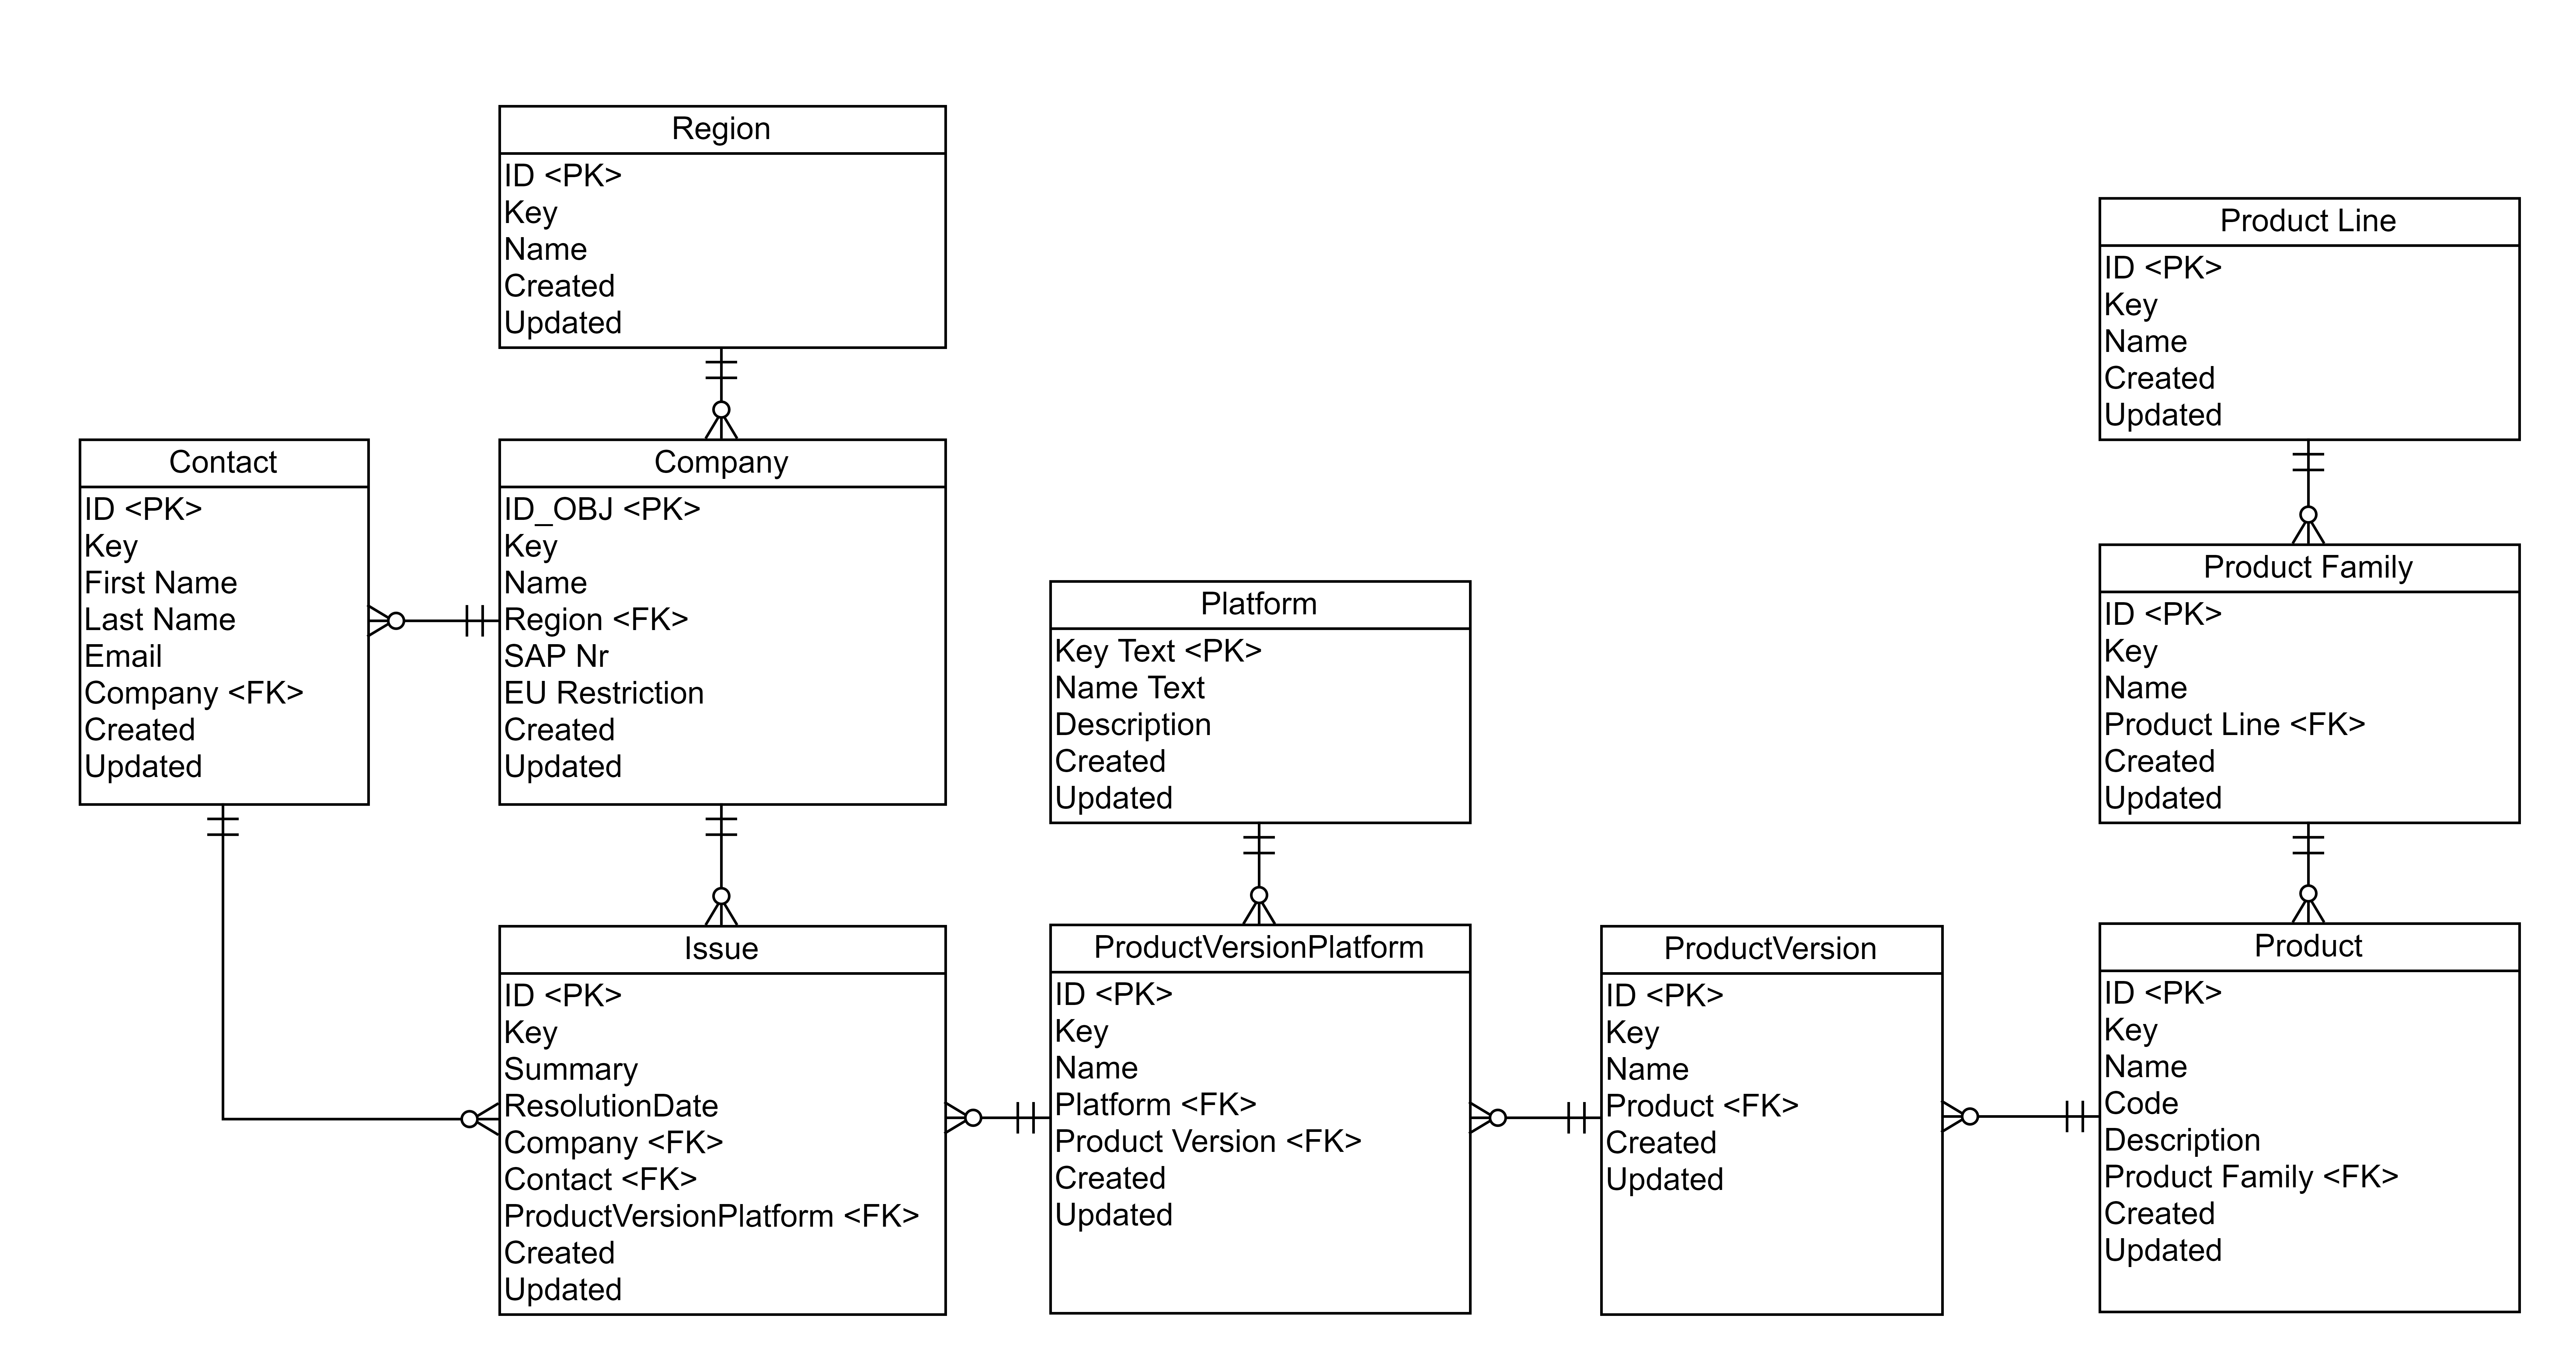
\includegraphics[width=\textwidth]{gfx/data_model.png}
 \caption{Verwendetes Datenmodell für den Prototyp}
\label{fig:praktischeUmsetzung:dataModel}
\end{figure}

\noindent Das gezeigte Datenmodell steht im Zusammenhang mit der Kundensupport-Software \textit{Jira Service Management}. Wenn ein Kunde (\textit{Company}) Probleme mit einem Produkt hat, wird von einer Kontaktperson (\textit{Contact}) ein Support-Ticket (\textit{Issue}) erstellt. Dabei werden alle notwendigen Produktinformationen wie Betriebssystem und Version mit dem \textit{Issue} verknüpft. Weitere Details sind an dieser Stelle nicht relevant.

% ================================================================================
\subsection{Datenbankmigration} \label{subsec:praktischeUmsetzung:Datenmigration}
Zu Beginn soll die Datenbank, die dem nachgestellten on-premise \acp{dwh} entspricht zu dem Cloud \acp{dwh} migriert werden. 

Für den Migrationsprozess wurden zwei Anwendungen betrachtet \cite{soh_microsoft_2020}: 
\begin{enumerate}
\item \textbf{\ac{dma}} ist ein Tool, das bewertet, wie gut eine Datenbank für die Migration in die Cloud geeignet ist und gibt einen Überblick, welche Funktionalitäten nicht übernommen werden können. Daneben gibt es die hier relevantere Funktion, das Datenbankschema und anschließend die Daten nach Azure zu übertragen. 
\item \textbf{Azure Database Migration Service} wird für Migrationen im großen Maßstab bevorzugt. Denn die Anwendung kann die Daten nicht nur von der on-premise Datenbank in eine Cloud Datenbank übertragen, sondern die Daten während und nach der Migration zwischen den beiden Systemen synchronisieren. Damit kann sichergestellt werden, dass neue Daten, die während dem Migrationsprozess gesammelt werden, nicht verloren gehen. Nach einer Übergangszeit wird die Synchronisation beendet. Diese Anwendung setzt jedoch voraus, dass das korrekte Datenbankschema bereits in der Zieldatenbank vorhanden ist und kann dieses nicht selbst übertragen. Daher wird eine Kombination mit dem \ac{dma} für ein vorheriges Importieren des Datenbankschemas empfohlen.
\end{enumerate}
Hier wurde sich für die Verwendung von nur \ac{dma} entschieden, weil eine Synchronisation der Daten während des Migrationsprozesses voraussichtlich nicht notwendig ist. Diese Annahme basiert darauf, dass in das on-premise BI-System nur einmal täglich neue Daten geladen werden und die Datenbankmigration nur einige Stunden dauert.

Die Durchführung beginnt mit der Installation des \ac{dma} auf dem gleichen Server wie die on-premise Datenbank. Für den Zeitraum der Migration wird die IP-Adresse der on-premise Maschine in den Firewall-Einstellungen des logischen SQL-Servers zugelassen. Anschließend wird der \ac{dma} geöffnet und der Migrationsprozess kann über die Benutzeroberfläche durchgeführt werden. Hierzu gehört die Angabe der Quell- und Zielserveradressen, Authentifizierungsinformationen und anschließend die Angabe der zu migrierenden Datenbank. Durch die Hub-and-Spoke-Architektur kann aus mehreren Datenbanken ausgewählt werden. Da sich alle Rohdaten in dem \textit{Hub}, welcher das \ac{dwh} abbildet, befinden, muss nur eine Datenbank migriert werden. Die \textit{Spokes}(Data Marts) werden nicht übertragen, weil diese für das aktuelle Reportingframework entworfen wurden, welches durch \textit{Power BI} abgelöst wird. Nach der Auswahl, wird automatisch ein SQL-Skript generiert, mit dem das Datenbankschema des \acp{dwh} importiert werden kann. Bei Bedarf kann das SQL-Skript angepasst werden und anschließend auf der Zieldatenbank ausgeführt werden, was nur wenige Sekunden gedauert hat. Abschließend können die Daten in die soeben erstellten Tabellen übertragen werden, wobei die Anwendung den prozentualen Fortschritt für jede Tabelle anzeigt. Die Übertragung von $1.3$ GB Daten hat ca. 50 Sekunden gedauert. Es kann also davon ausgegangen werden, dass die Migration der richtigen Datenbank(<500 GB) in deutlich weniger als einem Tag durchgeführt werden kann. Daraus folgt, dass der \ac{dma} nicht nur für den Prototyp ausreicht, sondern auch für die Migration des vollständigen \acp{dwh} geeignet ist.

Neben der Übertragung der Daten ist auch die langfristige Erhaltung der Datenqualität wichtig. Im on-premise SQL-Server werden hierfür Stored Procedures verwendet, welche über einen \textit{Job Agent} täglich ausgeführt werden. Diese führen Plausibilitätschecks durch und suchen nach Unstimmigkeiten, beispielsweise Duplikate oder ungültige Werte wie eine negative Bearbeitungszeit. Wenn eine Auffälligkeit gefunden wird, wird ein zuständiges Team per E-Mail benachrichtigt, sodass der Fehlerursache nachgegangen wird. Die Stored Procedures können problemlos als Bestandteil des Datenbankschemas migriert werden. Die \textit{Azure SQL Database} verfügt jedoch nicht über den \textit{Job Agent}, weswegen die regelmäßige Ausführung der Qualitätschecks anders gelöst werden muss. Eine naheliegende Lösung ist die Verwendung von \textit{Azure Functions}, da diese über einen Timer getriggert werden können, um dann die Stored Procedures auszuführen. Durch die Kombination mit \textit{Application Insights} können so gleichzeitig mit wenig Aufwand Logging der Qualitätschecks und Benachrichtigungen bei Problemen umgesetzt werden. Eine konkrete Umsetzung soll hier nicht vorgestellt werden, da die technisch relevanten Aspekte im Abschnitt zur Implementierung des \ac{etl}-Prozesses abgedeckt werden.

% ================================================================================
\subsection{Implementierung ETL}
Der ETL-Prozess mit \textit{Azure Functions} kann auf einer lokalen Maschine entwickelt und getestet werden, vorausgesetzt es können Quell- und Zielsysteme erreicht werden, die schematisch äquivalent zu den produktiven Systemen sind. Eine einfache Möglichkeit, um eine lokale Entwicklungsumgebung aufzusetzen, ist die Verwendung von Docker-Containern. Das Laden der Daten in das Zielsystem wird zum Beispiel mit dem \textit{Azure SQL Edge} Docker-Container getestet \cite[vgl.][]{msdoc_22_sql_docker}, der mit dem im letzten Abschnitt generierten Datenbankschema eingerichtet wird. In einer lokalen Datei werden die dazugehörigen Verbindungszeichenfolgen gespeichert und können in Code als Umgebungsvariable gelesen werden.

Bei den meisten Quellsystemen handelt es sich um Datenbanken, auf die aktuell direkt vom on-premise \ac{dwh} zugegriffen wird. Dabei sind die ETL-Prozesse mit T-SQL implementiert. Um den Migrationsaufwand zu verringern, wurde ein Konzept für \textit{Azure Functions} entwickelt, mit dem der Extraktions- und Transformationsteil der T-SQL-Abfragen nahezu unverändert übernommen werden kann. Gleichzeitig ist der C\#-Code so gestaltet, dass für unterschiedliche Entitäten nur eine andere T-SQL-Abfrage verwendet werden muss. Das Konzept für den ETL-Prozess zwischen zwei Datenbanken wird im Folgenden vorgestellt. Dabei gibt es durch die Infrastruktur keinen Unterschied zwischen on-premise und Cloud Datenbanken. 

Zum stündlichen Ausführen der Funktion wird über den Konstruktor die Verwendung eines \textit{TimerTriggers} mit einem \textit{NCrontab}-Ausdruck angegeben, sodass die Funktion zu jeder vollen Stunde aufgerufen wird. Im Konstruktor wird außerdem ein \textit{Logger-Objekt} übergeben. Alle damit geloggten Nachrichten werden an den Monitordienst \textit{Application Insights} übertragen.

Nach dem Aufruf wird zuerst ein Zugriffstoken geladen, welches notwendig für die Authentifizierung als \textit{Managed Identity} beim \ac{dwh} ist. Anschließend folgt der ETL-Prozess für jede Entität, deren Name in einem Array enthalten ist. Der Prozess ist in drei Schritte geteilt:

\begin{enumerate}
\item Frage aus dem Zielsystem den letzten Aktualisierungszeitpunkt der Entität ab.
\item Extrahiere und transformiere alle neuen oder veränderten Datensätze aus dem Quellsystem mit der zur Entität gehörigen T-SQL-Abfrage.
\item Lade die neuen Werte in das Zielsystem (Alle Aktionen werden innerhalb einer gemeinsamen Datenbanktransaktion ausgeführt):
    \begin{enumerate}[label*=\arabic*.]
    \item Erstelle eine temporäre Tabelle mit gleichem Schema wie Zieltabelle.
    \item Lade alle Daten mit Bulk-Copy in die Temporäre-Tabelle.
    \item Lösche alle Datensätze in Zieltabelle, die in der temporären Tabelle vorkommen.
    \item Füge alle Datensätze von temporärer Tabelle in Zieltabelle ein.
    \item Entferne temporäre Tabelle.
    \end{enumerate}
\end{enumerate}
Schritt 2 setzt voraus, dass in einem Unterverzeichnis für jede Entität eine gleichnamige SQL-Datei vorhanden ist. In der Datei steht die aus dem alten System übernommene SQL-Abfrage. In der WHERE-Bedingung wurde ein Parameter zum dynamischen Filtern der Datensätze nach ihrem letzten Aktualisierungszeitpunkt hinzugefügt. Der Quellcode kann im Anhang in Listing~\ref{lst:azFunc} gefunden werden.

Über den Editor \textit{Visual Studio Code} kann der Quellcode direkt nach Azure zu der \textit{Funktionsapp} übertragen werden. Die Verbindungszeichenfolgen zu den Quellsystemen, welche als Umgebungsvariable eingelesen werden, müssen dort noch hinzugefügt werden. Die sicherste Möglichkeit ist die Speicherung im \textit{Azure Key Vault}. Gespeicherte Geheimnisse im \textit{Key Vault} werden mit der \textit{Funktionapp} verlinkt, sodass sie als Umgebungsvariable verwendet werden können. Das Logging für den ETL-Prozess kann im Azure Portal über den Dienst \textit{Application Insights} gefunden werden. Dort wird eine Regel definiert, die an alle Benutzer in einer ausgewählten \ac{aad} Gruppe eine E-Mail-Benachrichtigung sendet, falls ein Fehler aufgetreten ist.

Insgesamt konnte bestätigt werden, dass der ETL-Prozess mit \textit{Azure Functions} funktioniert. Die Datenintegration von Quellsystemen über eine \ac{rest}-\ac{api} konnte ebenfalls erfolgreich umgesetzt werden, jedoch ist hier der Migrationsaufwand höher, da nichts aus dem on-premise BI-System übernommen werden kann und die Datentransformation in C\# erfolgen muss. Das Vorgehen ähnelt hier der Verwendung von \textit{Azure Functions} als Web-backend, weswegen es keine besonderen Ansätze gibt, die in dieser Arbeit erwähnenswert wären.

\cite[vgl.][]{kurniawan_practical_2019, satapathi_hands-azure_2021, sreeram_azure_2020}.

% ================================================================================
% Migration übernahme von Design
\subsection{Reporting}
Die Reports sind die Schnittstelle zum Endnutzer und präsentieren Auswertungen, die zum Planen und als Entscheidungshilfe genutzt werden können. Im neuen BI-System sollen diese mit \textit{Power BI} erstellt werden. Dabei soll \textit{Power BI} nicht nur für die Visualisierungen verwendet werden, sondern auch für Auswertungen und Transformationen, die vorher mit \textit{Data Marts} und \textit{T-SQL} durchgeführt wurden. Für den Umstieg zum neuen BI-System bedeutet dies, dass die Reports vollständig neu implementiert werden müssen. Nur eine erneute Gestaltung der Reports ist nicht erforderlich, sondern das aktuelle Design kann übernommen werden. Das ist sinnvoll, weil die Art, wie die Auswertungen dargestellt werden, bereits an die Wünsche und Bedürfnisse der Benutzer angepasst ist. Deswegen soll für den Prototyp ein Report erstellt werden, der hierfür alle relevanten Komponenten (Tabelle, Filter, Linien- und Balkendiagramm) enthält.

Der erste Schritt ist das Erstellen eines \textit{Datasets}, welches aus den Daten und dem Modell besteht. Dafür werden die Verbindungsinformationen zum \ac{dwh} angegeben und es wird die Option \textit{Import} gewählt. Der\textit{Import} bewirkt, dass das \textit{Dataset} in \textit{Power BI} zwischengespeichert wird und nicht jedes Mal neu generiert werden muss, wodurch die Performance signifikant besser als bei der Alternative \textit{DirecQuery} ist.

Nach dem Laden der Daten wird das Datenmodell mit dem \textit{Power Query Editor} bearbeitet. Zuerst wird die neue Spalte \textit{Alter} zu der Tabelle \textit{Issue} hinzugefügt. Das Alter für einen ungelösten \textit{Issue} ist die Zeit von Erstellung bis zum aktuellen Tag. Für einen gelösten ist es der Erstellungs- bis zum Lösungszeitpunkt. Ob ein \textit{Issue} in Bearbeitung ist, oder bereits gelöst wurde, kann abhängig davon, ob das \textit{ResolutionDate} gesetzt ist, erkannt werden. Dies wird mit einer IF-Funktion geprüft. Das erste Argument ist die IF-Bedingung. Ist die Bedingung wahr, wird das zweite Argument, ansonsten das dritte Argument ausgeführt. In beiden Fällen wird über eine Funktion die Zeitdifferenz in Bezug zum Erstellungszeitpunkt berechnet.

\begin{minipage}{\linewidth}
\begin{lstlisting}[caption=Code zur Defintion der Spalte \textit{Age} von Tabelle \textit{Issue},captionpos=b,style=sharpc]
Age = 
IF('issue'[ResolutionDate] = BLANK(),
    // Zeitdifferenz zum aktuellen Tag
    DATEDIFF('issue'[Created], NOW(), DAY),
    // Zeitdifferenz zwischen Erstellung und Lösung
    DATEDIFF('issue'[Created], 'issue'[ResolutionDate], DAY)
)
\end{lstlisting}
\end{minipage}

\noindent Beim Speichern der neuen Spaltendefinition wird jede Zeile der Tabelle automatisch um den neuen Wert ergänzt. Anschließend wird mit \textit{DAX} eine neue Tabelle \textit{Calendar} definiert, die jedes Datum vom Erstellungszeitpunkt des ersten \textit{Issues} bis zum aktuellen Tag enthält. Diese Daten werden hier für eine Zeitachse benötigt. Im nächsten Schritt ist es notwendig, die Beziehungen der Tabellen miteinander zu bearbeiten. Diese sind besonders für das korrekte Filtern in den Reports wichtig. Beziehungen können über die Benutzeroberfläche hinzugefügt werden, in dem Primär- und Fremdschlüssel und die Kardinalität angegeben werden. Nach der Bearbeitung entsprechen die Beziehungen in \textit{Power BI} dem Datenmodell in Abbildung~\ref{fig:praktischeUmsetzung:dataModel}. Damit ist das \textit{Dataset} bereit für die Verwendung in einem Report.

Als erstes Element wird ein Filter, \textit{Slicer} genannt, hinzugefügt, mit dem der Benutzer alle Visualisierungen interaktiv nach Region filtern kann. Dadurch, dass \textit{Power BI} die Beziehungen zwischen den Tabellen kennt, ist die Umsetzung sehr einfach und kann vollständig per Drag-And-Drop durchgeführt werden. Der \textit{Slicer} muss lediglich an die gewünschte Stelle gezogen werden und bekommt das Feld \textit{Name} von \textit{Region} zugewiesen. Jetzt kann ein Nutzer den Report per Dropdown-Filter auf eine Region beschränken.

Die manuell hinzugefügten Spalte \textit{Age} soll in einem Balkendiagramm verwendet werden, dass das durchschnittliche Alter eines \textit{Issues} nach Produktfamilie angibt. Dafür muss lediglich der Produktfamilienname als Achse und die \textit{Age}-Spalte für die Werte angegeben werden. Mit dem Setzen der Aggregationsart auf \textit{Durchschnitt} ist das Diagramm fertig.

Die nächste Visualisierung soll in einem Liniendiagramm den zeitlichen Verlauf der Anzahl an neu erstellten, geschlossenen und offenen \textit{Issues} anzeigen. Dazu werden der Tabelle \textit{Calendar} drei \textit{Measures} hinzugefügt. \textit{Measures} werden ebenfalls mit \textit{DAX} definiert und können für komplexere Aggregationen in den Visualisierungen verwendet werden. Im Gegensatz zu einer berechneten Spalte, wie \textit{Age}, werden die Ergebnisse von \textit{Measures} nicht im \textit{Dataset} gespeichert, sondern jedes Mal beim Laden des Reports neu berechnet. Diese Measures werden als Werte für das Liniendiagramm verwendet. Für die Achse werden nach Monat gruppierte Daten verwendet.

\begin{minipage}{\linewidth}
\begin{lstlisting}[caption=Measure: Anzahl neuer \textit{Issues} in einem Zeitabschnitt,captionpos=b]
New Issues = 
var startDate = MIN('Calendar'[Date])
var endDate = MAX('Calendar'[Date])
return CALCULATE (
    COUNTROWS(VALUES(issue[IssueID])), 
    FILTER(
        ALL(issue),
        issue[Created] >= startDate 
        && issue[Created] <= endDate 
        && (RELATED(region[Name]) IN VALUES(region[Name]))
    )
)
\end{lstlisting}
\end{minipage}

\noindent Mit der obigen \textit{Measure} wird für jeden Monat die Anzahl der neu erstellten \textit{Issues} berechnet. In Zeile 2 und 3 werden dazu das erste und letzte Datum des Monats in Variablen zwischengespeichert. Mit dem folgenden Ausdruck wird die Anzahl aller \textit{Issues} zurückgegeben, die eine Filterbedingung erfüllen. Der Filter verwendet in den Zeilen 8 und 9 die zuvor definierten Variablen, sodass nur \textit{Issues} in diesem Zeitraum gezählt werden. In Zeile 10 wird zusätzlich die Auswahl der Region im \textit{Slicer} berücksichtigt. Besonders benutzerfreundlich ist dabei die Funktion \textit{RELATED}, welche es erlaubt direkt auf den Namen der Region eines Issues zuzugreifen, obwohl dabei über zwei Relationen gegangen werden muss. 

Zuletzt wird noch eine Tabelle erstellt, die für jeden Kunden die Anzahl der offenen und geschlossenen Issues angibt. Dafür werden zwei Measures erstellt, die der vorherigen sehr ähneln und deswegen nicht genauer beschrieben werden. Erwähnenswert ist die Möglichkeit, diese beiden Measures in einer dritten zu verwenden, weil dadurch komplexere Berechnungen zerlegt werden können. Hier wurde zum Beispiel die Gesamtanzahl der erstellten Issues eines Kunden, durch die Addition der zwei anderen Measures berechnet.

\begin{minipage}{\linewidth}
\begin{lstlisting}[captionpos=b, caption={[Verwendung von Measures in Measure]Verwendung von Measures in Measure. Die Verwendung einer Measure unterscheidet sich nicht von einer normalen Spalte.}]
TotalIssues = 
company[OpenIssues] + company[ClosedIssues]
\end{lstlisting}
\end{minipage}

\noindent Abbildung~\ref{fig:praktischeUmsetzung:pbiRep} zeigt den fertigen Report.

\begin{figure}[htbp]
 \centering
 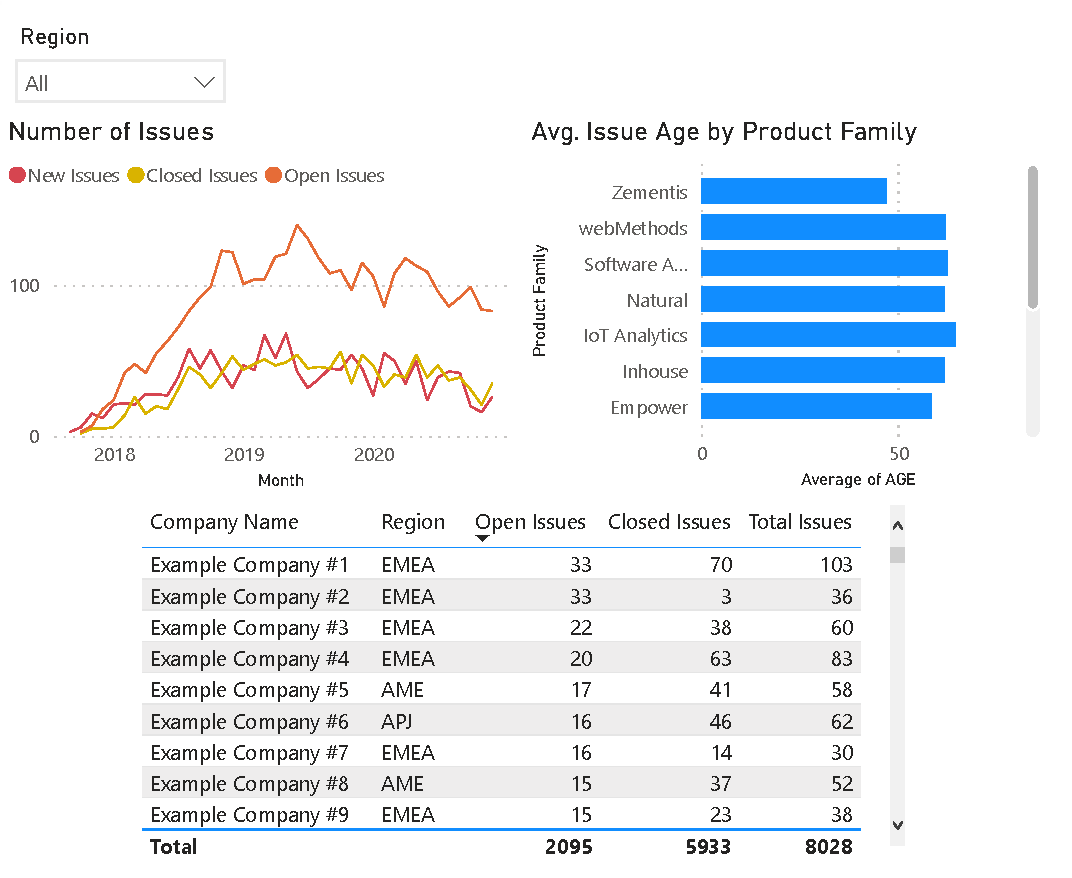
\includegraphics[width=\textwidth]{gfx/pbi_report.pdf}
 \caption[Power BI Report]{Mit Power BI erstellter Report (Anonymisiert und fiktive Zahlen)}
\label{fig:praktischeUmsetzung:pbiRep}
\end{figure}

Nach der Implementierung des Reports mit \textit{Power BI Desktop} kann dieser in einen \textit{Workspace} veröffentlicht werden. Danach ist der Report als auch das verwendete \textit{Dataset} für alle berechtigten Mitarbeiter über den Webbrowser verfügbar. Dort können diese nicht nur besichtigt werden, sondern beides kann für die eigene Verwendung heruntergeladen werden. Durch das Herunterladen des \textit{Datasets} muss beim Self-Service-Reporting weder eine Verbindung zu der Datenquelle aufgebaut noch eine Veränderung am Datenmodell vorgenommen werden. Dadurch wird das Erstellen von Reports erleichtert und einer deutlich größeren Benutzergruppe ermöglicht. Viele Visualisierungen können ohne Code per Drag-And-Drop erstellt werden, aber wie die Beispiele oben zeigen kann die Einarbeitung in \textit{DAX} sinnvoll sein, um das volle Potenzial von \textit{Power BI} zu nutzen.

Die Zugriffsberechtigung auf einen \textit{Workspace} kann über \ac{rbac} und dem \ac{aad} gesteuert werden. Falls eine granulare Zugriffskontrolle erforderlich ist, sollte jedoch die \textit{row-level security} verwendet werden. Mit dieser können Benutzern oder Gruppen \textit{DAX}-Filter zugeordnet werden, die einschränken, welche Inhalte gesehen werden können. Hier ermöglicht diese Funktionalität, dass der erstellte Report mit allen Mitarbeitern geteilt werden kann und gleichzeitig Daten, bei denen es durch die DSGVO notwendig ist, nur von Personen mit europäischem Standort gesehen werden kann.

Der letzte Schritt ist das Einrichten eines Zeitplans für die Aktualisierung des \textit{Datasets}. Dabei können auch E-Mail-Adressen angegeben werden, die im Fehlerfall benachrichtigt werden. Mit \textit{Power BI Pro} ist die Anzahl der Aktualisierungen auf achtmal täglich beschränkt, was bezüglich der Anforderungen der kritischste Nachteil gegenüber \textit{Power BI Premium} ist. Alternativ kann auch die Verwendung von \textit{DirectQuery} in Erwägung gezogen werden. \textit{DirectQuery} ist bei \textit{Power BI Pro} nicht eingeschränkt und lädt Daten direkt aus der Datenbank. Dadurch sind Reports immer aktuell, haben jedoch längeren Ladezeiten, da Transformationen und Berechnungen jedes Mal neu durchgeführt werden. Der Report in Abbildung~\ref{fig:praktischeUmsetzung:pbiRep} lädt beispielsweise mit \textit{DirectQuery} mehrere Minuten und ist damit über den maximalen 30 Sekunden Ladezeit, die in den Anforderungen festgelegt wurden. Daraus folgt, dass mit \textit{Power BI Pro} ein Report entweder die Anforderung an die Aktualität oder an die Ladezeit nicht erfüllen kann. Ob diese Einschränkung die zusätzlichen Kosten von \textit{Power BI Premium} rechtfertigt, ist fragwürdig, denn mit \textit{Import} konnten bezüglich der Performance keine Probleme festgestellt werden und das on-premise BI-System wird nur einmal täglich aktualisiert. Daher kann davon ausgegangen werden, dass \textit{Power BI Pro} mit dreistündlichen Aktualisierungen akzeptabel ist. Für Reports, bei denen die Aktualität besonders relevant ist, könnte außerdem eine zusätzliche Version, die \textit{DirectQuery} verwendet, bereitgestellt werden. Dann kann für jeden Einzelfall entschieden werden, ob der schnellere oder aktuellere Report benötigt wird. Sollte dieser Kompromiss zukünftig unzureichend sein, wäre außerdem der Umstieg zu \textit{Power BI Premium} jederzeit möglich.

\cite[vgl.][]{pearson_pro_2020}

% ================================================================================
\subsection{Einrichtung der Datengovernance} \label{sec:praktischeUmsetzung:purviewDatengovernance}
Zum Verwenden von \textit{Azure Purview} für die Datengovernance, muss der Dienst zunächst eingerichtet werden. Dazu öffnet ein berechtigter Nutzer die Webanwendung \textit{Purview Studio}. Als Erstes werden dort die Ressourcen, die gescannt werden sollen, registriert, indem die entsprechenden Verbindungsinformationen angegeben werden. Der Prototyp beschränkt sich hierbei auf das \ac{dwh}. Nun kann beim Erstellen eines sogenannten \textit{Scans}, die zuvor eingerichtete \textit{Self hosted-integration runtime} und die \textit{SQL-Database} angegeben werden. Daneben ist noch die Verlinkung mit dem Passwort des service principals im \textit{Key Vault} notwendig. Nach einem erfolgreichen Verbindungstest kann abschließend ein Zeitplan für regelmäßige Ausführungen des \textit{Scans} definiert werden, oder alternativ eine einmalige Ausführung gestartet werden. Während für den Prototyp letztere Option gewählt wurde, ist für ein zukünftiges Cloud-BI-System eine regelmäßige Wiederholung zu bevorzugen, damit die gesammelten Metadaten aktuell bleiben. 

Nachdem der \textit{Scan} durchgeführt wurde, können die gesammelten Erkenntnisse begutachtet werden. Dazu gehört zum Beispiel eine Übersicht über alle Tabellen und Spalten inklusive des Datentyps. Vom besonderen Interesse ist die Klassifizierung der Spalten, welche anhand einer Vielzahl von vordefinierten Regeln erfolgt. Diese Klassifizierungsregeln basieren entweder auf Wörterbüchern oder RegEx-Pattern und können damit unter anderem US-Sozialversicherungsnummern oder Bankleitzahlen erkennen. Auch das Hinzufügen von benutzerdefinierten Klassifizierungsregeln ist möglich. Kann der Wert einer Spalte zu einer Klassifizierungsregel zugeordnet werden, speichert \textit{Purview} eine entsprechende Klassifizierung, jedoch nicht den eigentlichen Wert. Für den Prototyp konnte damit eine einzige Klassifizierung gefunden werden, nämlich dass die Tabelle \textit{Contact} eine Spalte mit E-Mail-Adressen enthält. Hieran ist zu erkennen, dass die Klassifizierung grundsätzlich funktioniert, denn weitere Erkenntnisse waren bei dem vereinfachten Datenmodell nicht zu erwarten. Es muss jedoch angemerkt werden, dass diese Art von Klassifizierung sich nicht vollständig mit der dazugehörigen Anforderung deckt. In dieser wurde beschrieben, dass die  Daten bezüglich ihrer Vertraulichkeit klassifiziert werden sollen. Also nicht nach ihrem konkreten Inhalt, wie es bei \textit{Purview} der Fall ist. Dieses Problem könnte zum Beispiel durch die Funktion \textit{Sensitivitätskennzeichnungen} gelöst werden, welche sich aktuell in der Vorschauphase befindet. Da die Anforderung nicht die höchste Priorität hat und ein kurzzeitiger Ausfall der Funktionalität nicht kritisch für das operative Tagesgeschäft ist, wäre die Verwendung der Vorschau hier akzeptabel. Denn dann ist es möglich, basierend auf den gefundenen Klassifizierungen, automatisch \textit{Sensitivitätskennzeichnungen} zu den Metadaten hinzuzufügen. Wenn die Klassifizierungsregeln so festgelegt werden, dass aus bestimmten Kombinationen eine eindeutige Vertraulichkeit abgeleitet werden kann, wäre so ein vollständiges Erfüllen der Anforderung möglich.

Europäische Kunden verfügen über das \textit{Recht auf Vergessenwerden}, das innerhalb von 30 Tagen ausgeführt werden muss. \textit{Purview} kann sehr hilfreich sein, um alle Daten zu finden, die dann gelöscht werden müssen. In dem eine benutzerdefinierte Klassifizierungsregel angelegt wird, die bei eindeutigen Kundenkennzeichnungen greift, wie beispielsweise dem Namen oder der SAP-Nummer, können mit einem erneuten \textit{Scan} alle Tabellen und Reports mit Daten des Kunden gefunden werden. Dadurch wird das Risiko, dass Daten beim Durchführen der Löschung übersehen werden, minimiert.

Die von der DSGVO geforderte Datenflussdokumentation kann zwischen den Datenbanktabellen und den einzelnen Reports in \textit{Power BI} automatisch erstellt werden, in dem \textit{Power BI} als weitere Quelle für die \textit{Scans} registriert wird. Somit ist es möglich, schnell herauszufinden, welche Tabellen in welchen Reports verwendet werden. Die Datenintegration mit \textit{Azure Functions} wird allerdings nicht dokumentiert, da diese nur mit der \textit{Azure Data Factory} berücksichtigt werden kann. Demnach handelt es sich hier um eine weitere Anforderung, die mit Purview nur teilweise erfüllt werden kann. Aus diesem Grund \textit{Azure Functions} mit der \textit{Data Factory} zu ersetzen erscheint jedoch nicht sinnvoll, da dann weitere \acp{vm} notwendig wären, wodurch Kosten und Wartungsaufwand steigen. Da sich die Quellsysteme grundsätzlich selten verändern, wäre es voraussichtlich zeitsparender, die Dokumentation der Datenintegration manuell zu pflegen. Das ist über die \ac{rest}-\ac{api} von \textit{Purview} möglich. Dies würde immer noch den Mehrwert bieten, dass die vollständige Dokumentation aller Datenflüsse an einem Ort gefunden werden kann. Außerdem dürfen die meisten Nutzer Reports erstellen, während der ETL-Prozess nur von einer kleinen Gruppe verändert werden kann. Daher kann die Verwendung dieser Funktion insgesamt als positiv bewertet werden. 

\cite[vgl.][]{lesteve_definitive_2021, msdoc_22_purview_sensLabel, riscutia_data_2021, borosch_cloud_2021}

Zusammengefasst konnte durch die praktische Verwendung von \textit{Azure Purview} festgestellt werden, dass dieser Dienst einen guten Überblick über die Datenlandschaft im BI-System gibt und dadurch hilfreich beim Erfüllen von DSGVO-Vorgaben ist. Bezüglich der Anforderungen müssen allerdings Kompromisse, eingegangen werden, die durch die mangelnden Alternativen zu akzeptieren sind.